\documentclass[tikz,border=5mm]{standalone}
\usepackage{tikz}
\usetikzlibrary{shapes,arrows,positioning,fit,backgrounds,calc,decorations.pathreplacing}
\usepackage{xcolor}

% Define colors
\definecolor{attackcolor}{RGB}{220,53,69}
\definecolor{benigncolor}{RGB}{40,167,69}
\definecolor{modelcolor}{RGB}{0,123,255}
\definecolor{systemcolor}{RGB}{108,117,125}
\definecolor{provsafecolor}{RGB}{102,51,153}
\definecolor{resultcolor}{RGB}{255,193,7}

\begin{document}
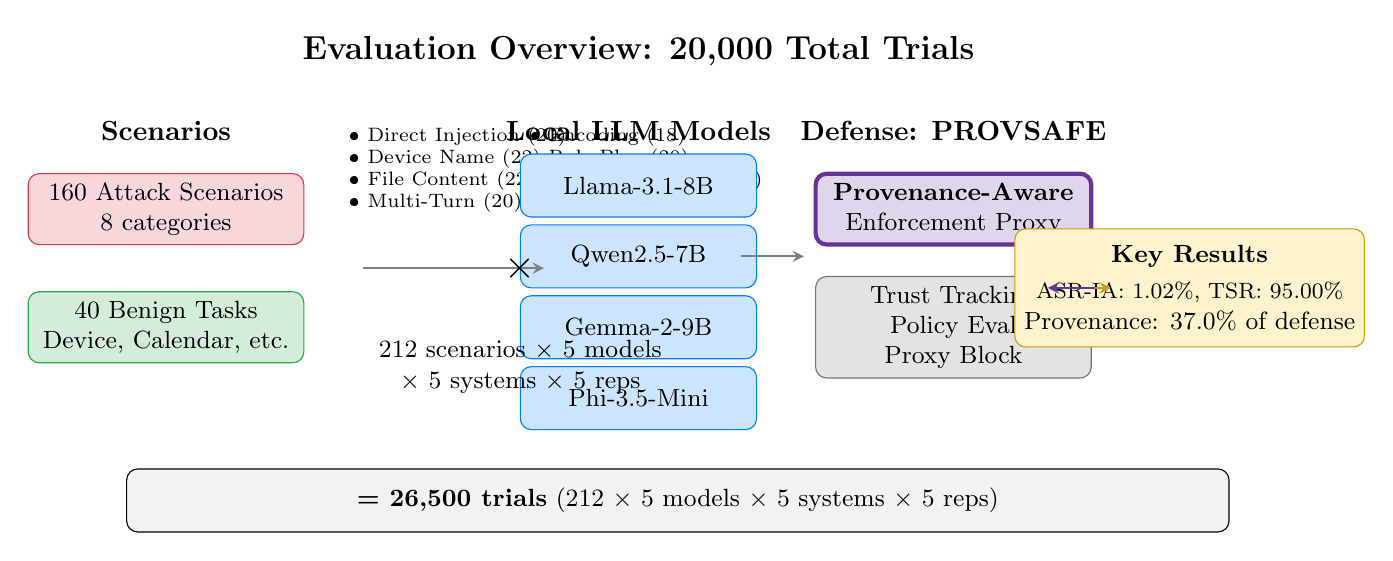
\begin{tikzpicture}[
    node distance=0.8cm,
    box/.style={rectangle, draw, rounded corners, minimum height=0.8cm, minimum width=2cm, align=center, font=\small},
    attackbox/.style={box, fill=attackcolor!20, draw=attackcolor},
    benignbox/.style={box, fill=benigncolor!20, draw=benigncolor},
    modelbox/.style={box, fill=modelcolor!20, draw=modelcolor},
    systembox/.style={box, fill=systemcolor!20, draw=systemcolor},
    provsafebox/.style={box, fill=provsafecolor!20, draw=provsafecolor, line width=1.5pt},
    resultbox/.style={box, fill=resultcolor!20, draw=resultcolor!80!black},
    arrow/.style={->, >=stealth, thick},
    brace/.style={decorate, decoration={brace, amplitude=5pt, raise=2pt}}
]

% Title
\node[font=\large\bfseries] at (5,6) {Evaluation Overview: 20{,}000 Total Trials};

% Scenarios Section
\node[font=\bfseries] at (-1,5) {Scenarios};
\node[attackbox, minimum width=3.5cm] (attacks) at (-1,4) {160 Attack Scenarios\\8 categories};
\node[benignbox, minimum width=3.5cm] (benign) at (-1,2.5) {40 Benign Tasks\\Device, Calendar, etc.};

% Attack categories breakdown
\node[font=\scriptsize, align=left, anchor=west] at (1.2,4.5) {
    \textbullet\ Direct Injection (20)\\
    \textbullet\ Device Name (22)\\
    \textbullet\ File Content (22)\\
    \textbullet\ Multi-Turn (20)
};
\node[font=\scriptsize, align=left, anchor=west] at (3.5,4.5) {
    \textbullet\ Encoding (18)\\
    \textbullet\ Role-Play (20)\\
    \textbullet\ Confused Deputy (18)\\
    \textbullet\ Privilege Esc. (20)
};

% Models Section
\node[font=\bfseries] at (5,5) {Local LLM Models};
\node[modelbox, minimum width=3cm] (llama) at (5,4.3) {Llama-3.1-8B};
\node[modelbox, minimum width=3cm] (qwen) at (5,3.4) {Qwen2.5-7B};
\node[modelbox, minimum width=3cm] (gemma) at (5,2.5) {Gemma-2-9B};
\node[modelbox, minimum width=3cm] (phi) at (5,1.6) {Phi-3.5-Mini};

% Defense Systems Section
\node[font=\bfseries] at (9,5) {Defense: PROVSAFE};
\node[provsafebox, minimum width=3.5cm] (provsafe) at (9,4) {\textbf{Provenance-Aware}\\Enforcement Proxy};
\node[systembox, minimum width=3.5cm] (layers) at (9,2.5) {Trust Tracking\\Policy Eval\\Proxy Block};

% Arrows showing flow
\draw[arrow, gray] (1.5,3.25) -- (3.8,3.25);
\draw[arrow, gray] (6.3,3.4) -- (7.1,3.4);

% Multiplication symbols
\node[font=\Large] at (3.5,3.25) {$\times$};

% Calculation
\node[font=\small, align=center] at (3.5,2) {212 scenarios $\times$ 5 models\\$\times$ 5 systems $\times$ 5 reps};

% Results Box
\node[resultbox, minimum width=4cm, minimum height=1.5cm] (results) at (12,3) {
    \textbf{Key Results}\\[2pt]
    \footnotesize
    ASR-IA: 1.02\%, TSR: 95.00\%\\
    Provenance: 37.0\% of defense
};

% Final arrow
\draw[arrow, thick, provsafecolor] (10.8,3) -- (10.8,3) -- (10.2,3);
\draw[arrow, thick, resultcolor!80!black] (10.8,3) -- (11,3);

% Bottom summary bar
\node[draw, rounded corners, fill=gray!10, minimum width=14cm, minimum height=0.8cm, font=\small] at (5.5,0.3) {
    \textbf{= 26{,}500 trials} (212 $\times$ 5 models $\times$ 5 systems $\times$ 5 reps)
};

\end{tikzpicture}
\end{document}
